%
% According to
% http://www.bth.se/tek/asb.nsf/sidor/31b58e62056523f7c12571a20027d9d3!OpenDocument
%
\documentclass[a4paper,oneside]{bthcsdiss}
%If you use Latex2.09 instead of Latex2e, comment the \documentclass line
%and uncomment one of the following lines (depending on whether you
%also want to use MakeIndex)

%\documentstyle[12pt,epsf]{illc_diss}
%\documentstyle[12pt,makeidx,epsf]{illc_diss}

%If you want to use MakeIndex, uncomment these lines
%\usepackage{makeidx}     % only with Latex2e
%\makeindex

\usepackage[utf8x]{inputenc}
\usepackage{tabularx}
\usepackage{natbib} % for funky \cite options
\usepackage{amsmath}
\usepackage{mathenv}
\usepackage{amssymb}
\usepackage{amsthm}
\usepackage{textcomp}
%\usepackage{a4wide}
\usepackage{longtable} %table spanning pages
\usepackage{multirow}
\usepackage{pifont}
\usepackage{changepage}
\usepackage[font=small,labelfont=it,bf]{caption} %for customizable figure and table captions

\usepackage{fancyhdr}  % you can choose between 7 different types of heading, besides the default. for instance, try 
%\usepackage[Lenny]{fncychap} 
%\usepackage[Conny]{fncychap}
%\usepackage[Sonny]{fncychap} 

%\usepackage{algorithmic}
%\usepackage{algorithm}
\usepackage{listings}
\usepackage{url}
\usepackage{xspace}
\usepackage{xtab}
% \usepackage{palatino} %for different font type
% \usepackage[T1]{fontenc}
%\usepackage[scaled]{uarial}% for the modern-look fonttype:
%\renewcommand*\familydefault{\sfdefault}

%\usepackage{soul, color} % this with the next one gives convenient colouring options for drafts, e.g. with a \hl{xxx}, the marking becomes ugly green.

%\sethlcolor{green} 
%\setul{2pt}{0.5pt} % use this if you want to change spacing of the underling

\usepackage[neveradjust]{paralist} %this one is handy if you are short on space or want to have a listing with bulletes, starts etc. e.g. use \begin{compactenum} \item ... \end{comactenum}

%\usepackage[top=3cm, bottom=2.8cm, left=2.7cm, right=2.7cm]{geometry} % to make nice page margins to squezze more or less text on a page

% *** GRAPHICS RELATED PACKAGES ***
%
\usepackage{graphicx}
% declare the path(s) where your graphic files are
\graphicspath{{figures/}}
% and their extensions so you won't have to specify these with
% every instance of \includegraphics
\DeclareGraphicsExtensions{.pdf,.png}

\usepackage[bookmarks=true,%
bookmarksopen=true,%
bookmarksopenlevel=0,%
bookmarksnumbered=true,%
colorlinks,%
linkcolor={black},%
citecolor={black},%
urlcolor={black},%
pdfstartview={FitV},%
unicode,%
breaklinks=true,%
plainpages=false,%
%TODO set title
pdftitle={TITLE},%
pdfauthor={Matteus Magnusson and Suresh Balsasubramaniyan}]{hyperref}

%%%%%%%%%%%%%%%%%%%%%%%%%%%%%%%%%%%%%and then my shortcuts

% put your \newcommand etc here. For instance, the following formats are quite nice, but you also can take the default by commenting them:

% \newtheorem{lem}{\textsc{Lemma}}[chapter]
% \newtheorem{thm}{\textsc{Theorem}}[chapter]
% \newtheorem{prop}{\textsc{Proposition}}[chapter]
% \newtheorem{post}{Postulate}[chapter]
% \newtheorem{corr}{\textsc{Corollary}}[chapter]
% \newtheorem{defs}{\textsc{Definition}}[chapter]
% \newtheorem{cons}{\textsc{Constraint}}[chapter]
% \newtheorem{ex}{\textbf{Example}}[chapter]
% \newtheorem{qu}{\textbf{Question}}[chapter]

%\makeindex

%\typeout{bth CS Dissertation Example File `guide.tex' <June 23, 2007>.}

%%%%%%%%%%%%%%%%%%%%%%%%%%%%%%%%%%%%%%%%%%%%%%%%%%%%%%%%%

\begin{document}
\pagenumbering{alph}

\pagestyle{plain}

%%%%%%%%%%%%%%%%%%%%%%%%%%

%%  \include the `front matter'

% !TEX root = ../main.tex
% !TEX spellcheck = en_US
%% This is the standard `front matter' to be used with the illcdiss.cls
%% Latex2e document class or the illc_diss.sty Latex2.09 style file
%%
%%
%% MAKE SURE THAT THE FILE HAS BEEN PERSONALIZED BEFORE YOU
%% PRINT AND SHIP THE FINAL VERSION.  YOU CAN FIND ITEMS THAT NEED
%% TO BE PERSONALIZED BY SEARCHING FOR THE STRING ``%PERSONALIZE''
%%
%%
%%first of all the cover.
{\pagestyle{empty}
\changepage{5cm}{1cm}{-0.5cm}{-0.5cm}{}{-2cm}{}{}{}
\noindent%   
{\small
\begin{tabular}{p{0.735\textwidth} p{0.21\textwidth}}
\textit{Master Thesis} & \multirow{7}{*}{\bthcslogo{3.22cm}} \\
\textit{Computer Science}\\
\textit{Thesis no: MCS-2012-97}\\ %TODO set thesis number
\textit{09 2012} \\ %TODO set month
\end{tabular}}

\begin{center}
%\line(1,0){400} %as you like
\par\vspace {7cm}

{\Huge\textbf{A Communicating and Controllable Teammate Bot for RTS Games}}   %PERSONALIZE 

\par\vspace {0.5cm}

{\Large\textbf{in StarCraft}}   %PERSONALIZE
\marginpar{Any good subtitle?}

\par\vspace {3cm}
%{\Large\textbf{Irene Moriggl}}
%\par\vspace {0.5cm}
{\Large\textbf{Matteus M.\ Magnusson\\\vspace{0.25em}Suresh K. Balsasubramaniyan}}
\par\vspace {7cm}
%This thesis is presented as part of Degree of\\
%European Master in Software Engineering 

%\par\vspace {2cm}
%Blekinge Institute of Technology\\
%June 2010

%\line(1,0){400} %as you like
\end{center}

\noindent%
{\small School of Computing\\
Blekinge Institute of Technology\\
SE-371 79 Karlskrona\\
Sweden}

\clearpage
}

{\pagestyle{empty}
\changepage{5cm}{1cm}{-0.5cm}{-0.5cm}{}{-2cm}{}{}{}
\noindent%
{\small This thesis is submitted to the School of Computing at Blekinge
Institute of Technology in partial fulfillment of the requirements for the degree of Master
of Science in Software Engineering. The thesis is equivalent to 20 weeks of
full time studies.}
\par\vspace {12cm}

\noindent%
\begin{tabular}{p{0.5\textwidth}lcl}
\textbf{Contact Information:}\\
Authors:\\
Matteus M.\ Magnusson\\
E-mail: \href{mailto:matteus.magnusson@gmail.com}{matteus.magnusson@gmail.com}\\
\par\vspace {0.5em}
Suresh K.\ Balsasubramaniyan\\
E-mail: \href{mailto:suresh.draco@gmail.com}{suresh.draco@gmail.com}\\
\par\vspace {4cm}
%\par\vspace {5cm}
University advisor:\\
Dr.\ Johan Hagelbäck\\
School of Computing
\par\vspace {1cm}
\noindent%
School of Computing \\
Blekinge Institute of Technology & Internet & : & www.bth.se/com\\
SE-371 79 Karlskrona & Phone	& : & +46 455 38 50 00 \\
Sweden & Fax & : & +46 455 38 50 57 \\
\end{tabular}
\clearpage
} % Back to \pagestyle{plain}

%%%%%%%%%%%%%%%%%%%%%%%END of FRONT MATTER%%%%%%%%%%%%%%%%%%%%%%%%%%%
\pagenumbering{roman}
\begin{abstract}
	This thesis evaluates if a teammate bot, in Real-Time Strategy (RTS) games, can be used as a tool to
create new experiences. The bot extends an existing bot in StarCraft: Brood War; the bot
functions more or less as a human player, but the player gives it high-level commands about tactics and
strategies. To test the bot, it comes with three degrees of initiative: low, medium, and high; the player is asked to
play with all. When the bot is implemented players evaluate the bot by playing with it and then interviewed about their
opinions on the bot.
\end{abstract}

%\include{acknowledgments} %OPTIONAL
%\listoffigures %in case you have them
%\listoftables %in case you have them
%\listofalgorithms %in case you have them
\tableofcontents 

%%  now we can start with the real thing

\cleardoublepage
\pagestyle{headings}
\pagenumbering{arabic}
% !TEX root = ../main.tex
\chapter{Introduction}
Have you ever wanted to be the boos over your teammate bot\footnote{A bot is a computer player that you either can play with or against} in a game? No!? Then you can stop reading. Today you can find a few new Real-Time Strategy (RTS) games, but none of these lets you control your teammate bot, let alone collaborate with it, at least not to our knowledge; this includes research, where we have not found a single subject on communication between human player and bot.

The focus lies in evaluating if it is worthwhile to do further research in this unexplored area, both for the purpose of researchers and for game developers to help them decide if they shall invest money in a collaborative teammate bot for RTS games.

To familiarize you with the subjects presented a brief description on all subjects are given below. Once you have basic knowledge of the subjects we will give a thorough background what others have done in closely related subjects. Next a detailed description of the methods we used are described; this includes implementation on the bot, why it was implement this way, and how it was evaluated. 
%: Rephrase
The evaluation results are then presented, at the end we conclude the results and presents new subjects of future work.

\section{RTS}
An RTS game is a computer game that heavily relies on strategy and fast executing. An analogy would be to play chess where both you and your opponent can move pieces at the same time, you will only see your own pieces and a tile beside them; meaning you do not know the location of the opponent’s pieces or when s/he makes a move, on top of that you have to think of a strategy fast before your opponent gets a lead.

In reality, RTS games resembles more a battle field than a game of chess—you control the army and it’s unit and on what the resources shall be spent on. From the start of the game you have a single base and your goal is to build up the technology to create powerful units by collecting resources, but you cannot go straight for the best technology because it takes time and if the opponent comes with any attack you will be defenseless against it.

There is no real standard how RTS games they all work a bit different but have the
%: Continue here

and a set of workers, these workers can build structures and collect resources—used to build structures, upgrades, and units. Various games have collects and build structures in different ways, some games does not use workers for building buildings, and some gets resources from buildings placed at specific points.
%: Find source for games that doesn’t use workers for gathering resources

%: Import a StarCraft image

\subsection{StarCraft}
The AI is implemented in an RTS game: StarCraft, more specifically StarCraft : Brood War—an expansion to StarCraft that introduced new units. Henceforth StarCraft: Brood War will be referenced as StarCraft for simplicity..


\subsubsection{Gameplay}
StarCraft has three races—Terran, Protoss, and Zerg—which the player can choose from. Each of these races have their own unique type of units and their playstyles are very different to each other.

\paragraph{Commonalities between races}
Common for all races is that they all have a worker unit that collects minerals and gas—minerals and gas are the games resources used to build structures, units and upgrades. Minerals and gas are usually located in clusters where the player can build a base. This makes the distance short from the resources to the base which all resources has to be carried to. Only one worker can simultaneously collect minerals from a mineral field, or gas from a gas depot. Minerals have a fixed number of resources to them that can be mined before they disappear; gas on the other hand too have a number of resources, but after that limit is reached gas can still be mined, but now the worker only harvest 2 gas instead of 7. To harvest gas a structure needs to be built on top of the gas depot.

Each unit occupies an amount of supply, ranging from a half supply (Zerglings) to 8 supplies (Carriers). Zerg's Overlord is the only unit that doesn't take any supplies, in fact it gives supplies, this is described in the following text. The maximum supply of units is 200 for all races. To get more supplies than the starting amount, the races have to either build a new base structure or a special supply structure, or unit in the Zerg's case.

\paragraph{Terran}
Terran's worker unit 'SVC' can repair structures, and vehicle units. When they construct a structure they becomes occupied with that task and cannot do anything else. The SVC can however abort the building and let another SVC continue with the construction.

While Protoss's supply structure and Zerg's supply unit has special abilities the Terran's supply unit does nothing more than take up place and give 8 supply to the player.

\paragraph{Protoss}
Protoss units and structures have two health bars oppossed to Terran's and Zerg's one health bar. The first health bar is the base health of the unit, the other is a shield that recharges ones the unit or structure is out of battle. This makes the units and structures strong against small attacks that only damage the units shields, since they can retreat and regain full health again. Note that not all occaissions allow this, since the enemy is usually reluctant to let a protoss army flee to regain full health.

Protoss's worker unit 'Probe' can only mine resources and summon structures, it cannot repair any units as Terran's SVC can. While SVC's are occupied the whole time they construct structures a Probe can simply start to summon a building and it will construct itself. Protoss structures, however, has one restriction, structures needs to be placed under the power of a pylon, pylons are Protoss supply structure and power source. A pylon emits a circle of power and if a structure becomes powerless—the pylon has been destroyed—it will not function and a new pylon has to be built. Pylons, Nexuses (Protoss base), and Assimilator (gas structure) can function without a pylon.

\paragraph{Zerg}

\subsubsection{Balanced}

\section{Teammate}

\subsection{Player}

\subsubsection{General}

\subsubsection{RTS}

\subsection{AI}

\subsubsection{General}

\subsubsection{RTS}

\subsection{Voice Communication}
\section{Background}
Up to date there has, as we know of, been little research for teammate bots\footnote{A bot is a computer player that
you either can play with or against.}; this is especially true for Real-Time Strategy (RTS) games, where only one
scientific article\cite{abraham_ai_2010} was found. There do however exist other articles\cite{jansen07,taylor08} on the
subject. The bots in these articles neither adapts their behavior nor do they convey their intentions to the human
player through communication. There exists other articles on the subject of teammate bots, independent of genre; Tan and
Cheng writes about teammate bots adapting to other teammate bots\cite{Tan_Cheng_2007, zhou_pucheng_multi-agent_2011};
Simon writes about teammate bots in general\cite{simon07}.

To beat the enemy in an RTS game, as a team or one player, you need a strategy that exploits the enemy's weaknesses as
the time while eliminating your own weaknesses. If your strategy is bad, it does not matter how hard you try to win, you
will still loose—don't try to spike a nail with a feather. Articles on player modeling include complementing the
teammate player's weaknesses\cite{jansen07, houlette03, zhou_pucheng_multi-agent_2011} and finding the enemy's
weaknesses\cite{kabanza_opponent_2010, synnaeve_bayesian_2011, schadd_opponent_2007}.

One article\cite{McGee:2010:RTA:1822348.1822365} mentions something the communication between the human player
and the bot (for any genre); the survey article concludes that ``little or no work'' has been done on ``concept learning
and clustering (\ldots), inferencing, and communication''; we verify this by not finding a single subject on
communication for any genre, let alone RTS games.
\chapter{Problem description and problem statement}
% !TEX root = ../main.tex
\chapter{Methods}

% !TEX root = ../../main.tex

We begin by describing the main features, behaviors, and goals of our bot; these features have been selected by either what players wanted, 0what we think would be a good feature, or both and then testing what works and what does not. We then give a brief overview of the system and how the different components/classes work and communicate with each other to get a quick grasp how everything is connected.

After the overview we will give a detailed description of all the important features of the classes, giving motivations of our design choices. The design choices were selected by either research, common knowledge in the StarCraft community, what we think would be good, or a mix of any and then testing what works and what does not, first on ourselves and then, close to the end, on our test players to find weird and non-acceptable behaviors.

\paragraph{Configurable variables}
Many fixed variables in BATS are configurable from a config.ini file. This design choice was made to easily tweak these variables in-game, instead of having to recompile, start the game, wait until the game state is present (necessary buildings have been built). The configuration file could be reloaded anytime in-game using \emph{/reload config} command. Throughout the method section these will be presented with their current value, variables that are configurable will have a superscript of \conf attached to it, e.g. 150\conf seconds. If a range has a superscript, e.g. [0.0, 1.0]\conf both 0.0 and 1.0 is configurable.
% !TEX root = ../../main.tex
\section{Build planner}
Build planner is the core for planning Structure (Building) and Army creations. Here Building or Structure includes production, upgrade, add-on and resource gathering buildings and Army refers to all combat and non-combat (Medic) type units.
The production process during the whole game is divided into three phases namely early, mid and late. BATS follows specific build order provided in the configuration file (/BATS-data/buildorder/) by the user. User can configure and keep more than one build order for a phase. The exact transition graph is configured using "transition" config file and the individual phase build order is configured using files in early, mid and late folders.
The phase transition during the game is done by the command "transition" or "transition FILE_NAME". The configuration in the "transition" file is overriden by the command "transition FILE_NAME". BATS asks user for the permission to make transition in case if the user forget to do so.
The priority of the production is the order in which the units are placed in the configuration file. The Army is classified into "Must Have" and "Percentage" units for each phase. The priority of army production is done based on maintenance of percentage and higher priority is given to the "Must Have" units over "Percentage" units.
E.g. format
<name>
early-x
<available-transitions>
mid-x
mid-Y
<build-order>
Terran_Supply_Depot
Terran_Barracks
Terran_Refinery
Terran_Bunker
Terran_Academy
Terran_Factory
<units>
80% Terran_Marine
20% Terran_Medic
<must-have>
2 Terran_Medic
1 Terran_Vulture

Above is the default configuration followed by the BATS for phase "early-x" which can be edited by the user. Separate configuration is available for separate phase namely "early", "mid" and "late". The configuration file has three parts name, available-transition, build-order, units and must-have. <name> has the phase name to which the configuration file applies to. <available-transition> has the possible phases to which the current phase can transit to. <build-order> has the list of structure or building names to be built for that phase. The structures are built in the order they are listed. <units> defines the Army that the current phase should have and is mentioned in percentage. 
It will always prioritize the unit that is furthest away from its goal.
E.g. 60% marines are at (56%), 20% tanks are at (18%) will choose to prioritize a tank, why?
Marines: 56/60 = 0.933... meaning roughly 7% from its goal.
Tanks: 18/20 = 0.9 meaning 10% from its goal.
Tanks are then furthest away from its goal.
<must-have> lists the units that are compulsory to be available during a phase. Units are listed in decimal numbers. If the highest priority unit cannot be built because of: 
- Low minerals -> Wait for minerals, do not build another unit
- No buildings are free (or does not exist) -> Build next unit in the priority list instead.
BATS maintains the production by considering the unit destruction and building availability to produce that unit. i.e. when a must have unit is destroyed, it is rebuilt again and when a percentage unit is destroyed, it is added again into the production queue.
BATS has pre-defined or default set of configuration for each phase and the transition. Following is the example or format how the transition config file should be.
E.g. early-x>mid-y>late-z
% !TEX root = ../../main.tex
\section{Squads}
% !TEX root = ../../main.tex
% !TEX spellcheck = en_US
\section{Commander}
\label{sec:Commander}
The Commander creates all orders for BATS, except defenses as the \nameref{sec:defense_manager} does
that. This means that it orders attacks, drops, expansions, scouts, and when to transition to the
next phase.

\subsection{Orders/Commands}
Below are all orders that both BATS can decide to use (described further down) and the teammate can
order through his commands. The commands almost behave exactly the same independent on who ordered
the command except that if a command fails it will only print out an output if the teammate ordered the
command—some other exceptions exist.

The orders work differently depending on the current state of BATS. Because of all tests and
different behaviors in the commands, these are easily described in pseudo-code. Common for all
functions are the two parameters: \texttt{teammateOrdered}
and \texttt{reason}; teammateOrdered is set to true if the teammate ordered the command, reason is
the reason to print out if the command is successful, the reason parameter is only used when BATS ordered the
command—e.g. attack because BATS expands. The messages are sent with the help of
\texttt{IntentionWriter}; how IntentionWriter works is described in section \ref{sec:communication}.

\paragraph{Attack}
Has in general three behaviors: Creates a new frontal attack, reinforces the existing frontal
attack, or does nothing. Listing \ref{lst:order_attack} displays the pseudo-code for the attack
command.
\begin{lstlisting}[label={lst:order_attack},caption={Pseudo-code for the attack command}]
// Never do a frontal attack when under attack
if (isUnderAttack()) {
	if (teammateOrdered) {
		IntentionWriter.write(BotAttackNot, BotIsUnderAttack);
	}
	return;
}

// Teammates can create attacks even if few units
if (teammateOrdered) {
	canAttack = !freeUnits.empty();
} else {
	canAttack = canFrontalAttack(); // Checks enough units
}

if (canAttack) {
	oldSquad = mSquadManager.getFrontalAttack();
	
	// Add free units to the old Attack squad if it exists
	if (oldSquad != NULL) {
		oldSquad.addUnts(freeUnits);
		IntentionWriter.write(BotAttackMerged, reason);
	}
	// Create new attack and ping position
	else {
		attackSquad = new AttackSquad(freeUnits);
		attackPos = attackSquad.getAttackPosition();
		IntentionWriter.write(BotAttack, reason, attackPos);
	}
} else {
	IntentionWriter.write(BotAttackNot, BotNotEnoughUnits);
}
\end{lstlisting}

\paragraph{Follow}
Follow almost behaves as the attack command, but instead of creating a regular Attack squad, it will
instead follow the largest teammate player’s squad. In addition to the attack’s three
behaviors—create new frontal attack (that follows teammate), reinforce the frontal attack, or does
nothing—it has one additional behavior: If BATS already has a frontal attack, that is not following
a teammate, it will abandon its goal and instead follow the teammate.

\paragraph{Drop}
Drop will try to create a drop from any of the unit compositions that are available.
\begin{lstlisting}[label={lst:order_drop},caption={Pseudo-code for the drop command}]
availableCompositions = getUnitCompositionByType(freeUnits, Drop);

// Create drop
if (!availableCompositions.empty()) {
	randomId = rand() % availableCompositions.size();
	chosenComposition = availableCompositions[randomId];

	drop = new DropSquad(freeUnits, chosenComposition);
	IntentionWriter.write(BotDrop, reason, drop.getDropPosition());
}
// No drops available
else {
	if (teammateOrdered) {
		IntentionWriter.write(BotDropNot, BotNotEnoughUnits);
	}
}
\end{lstlisting}

\paragraph{Scout}
As with drop, scout uses available unit composition; it does however not choose a random composition
but uses the composition with highest priority—i.e. the first composition, as
UnitCompositionFactory’s getUnitCompositionByType() returns composition sorted by priority, where
the highest priority is first.

\paragraph{Expand}
Expand will first check if there are any expansions available, i.e. not already taken; if there are
expansions available it will append a command center (or equivalent for other races) to the Build
planner, which in turn will build an expansions when it has resources for it.

\paragraph{Transition}
Transition transitions to the next phase in the game—there are three phases: early, mid, and late
game. How the Commander handles the transition command can be seen in listing
\ref{lst:order_transition}.

\subsection{Order creation rules}
The Commander can create orders either from its own actions and states, or what the teammate player
is doing. Examples of this is it might attack when it is expanding, and it might expand if it has
high amount of minerals, for reaction to teammate actions it attack if the teammate player is
expanding.
\clearpage
\begin{lstlisting}[label={lst:order_transition},caption={Pseudo-code for transition command}]
// Only transition if not in late game already
if (mBuildPlanner.canTransition()) {
	if (mBuildPlanner.getCurrentPhase() == "early") {
		intention = BotTransitionMid;
	else if (mBuildPlanner.getCurrentPhase() == "mid") {
		intention = BotTransitionLate;
	}

	mBuildPlanner.switchToNextPhase();
} else {
	if (teammateOrdered) {
		IntentionWriter.write(BotTransitionNot, BotTransitionNoMore);
	}
}
\end{lstlisting}

\subsubsection{Reacting on own actions and states}
\label{sec:react_own}
These are the reactions (commands) to BATS's own state.

\paragraph{Expand}
In order to expand from own reactions BATS needs to meet all conditions below.
\begin{itemize}
  \item \textbf{Not be under attack.} Expanding when we are under attack will most likely kill the expansion
	  directly
	\item \textbf{Not already be expanding.} We do not want to spam expansions
	\item \textbf{Less than \CommanderExpansionActiveMax~active expansions.} Good number of
	  active bases as it keeps a large and steady income to support many unit producing structures.
	  Active expansions are expansions where at least
	  \classificationExpansionExpansionMineralsLow~minerals left.
	\item \textbf{No new expansion shall have been build in \CommanderExpansionIntervalMin.} Again we do not
	  want to spam expansions and this seemed like a reasonable time, but has not been extensively
	  tested.
\end{itemize}
When all four conditions are met it will check if any of the following conditions are met, if they
are an expansion will be added to the beginning of the build order.
\begin{itemize}
	\item \textbf{BATS is attacking.} It is good to expand when attacking (or vice versa) as this
	  distracts the enemy from the expansion long enough for the expansion to complete\cite{day9}
	\item \textbf{Expansions are saturated.} This tests if the number of workers per mineral patch is at or
	  above \classificationExpansionWorkersPerMineralSaturation. Simply put, even if you add more
	  workers to mine, they will have to wait longer for the mineral patch to be free, thus it will
	  not increase your income. This rule will allow BATS to expand early in the game when it has
	  less than \CommanderExpansionActiveMax~expansions.
	\item \textbf{An expansion is running low on minerals.} Making sure we stay on the same number of active
	  expansions. This is the same as an expansion that is not active (i.e. having less than
	  \classificationExpansionExpansionMineralsLow~minerals left) but still having some minerals
	  left to be mined.
	\item \textbf{High on minerals.} If we have too much minerals that means we cannot build enough structures
	  or units, thus we can as well add another base and possibly increasing the amount of gas
	  mined. Activates when the mineral count is above \classificationHighOnMinerals.
\end{itemize}

\paragraph{Attack}
To attack from own reactions BATS shall meet all conditions below.
\begin{itemize}
  \item \textbf{Shall not be under attack.} It is better to stay and defend and then possibly
	attack, although a small counter-attack might be effective when the enemy army is small and BATS
	can spare some units for the attack, counter-attacks have not been implemented.
  \item \textbf{Not have a current attack.} Having one big army is easier to control and generally
	much stronger than splitting it into 2 smaller attacks for slower armies\cite{day9}, and BATS will
	use slower armies in the experiment. Although ordering a second attack when we have a frontal attack will
	reinforce units, but we did not have enough time to implement and test when to reinforce the
	army.
\end{itemize}
When all two conditions are met it will check if any of the following conditions are met, if they
are an attack will be created.
\begin{itemize}
	\item \textbf{Expanding.} As explained earlier under the expand, it is good to attack while
		expanding.
	\item \textbf{Upgrade soon done.} When an upgrade will finish soon this means that the bot will
		get stronger and it might be possible that the enemy has either not caught up in upgrades, i.e.
		the longer we wait the less valuable the upgrade is\cite{day9}. Upgrade soon done checks if any
		of the free units that could be used for an attack will be affected with an upgrade that is
		currently upgrading and if the upgrade finishes within \classificationUpgradeSoonDone.
\end{itemize}

\paragraph{Scout}
The scout order conditions are much simpler than expand and attack. BATS will always send out a
scout if it is not scouting, not under attack, and has \CommanderScoutOnWorkerCount. The Commander
uses \nameref{sec:unit_composition}s for the scout to get the best available scout unit. From lowest
priority this is:
\vspace{0.5em}
\begin{compactenum}
  \item SCV
	\item Marine
	\item Vulture
	\item Wraith
\end{compactenum}
Wraiths are flying units with cloak ability (if researched) this make them an ideal scout as they
fly over terrain, are quite fast, and can cloak if they get too close to the enemy. Vultures are on
the other hand the fastest ground unit for Terran. See section \ref{sec:scout_squad} how squads
work, listing \ref{lst:unit_comp_scout} for the unit composition config file, and
\ref{sec:unit_composition} for how unit compositions work.

\paragraph{Transition}
The transition order conditions are just as simple as the scout. It will transition if it is not
already in late game, no buildings in the build order, and is high on resources (higher or equal to
\classificationHighOnMinerals~minerals and \classificationHighOnGas~gas).

\subsubsection{Reacting on teammate actions} All orders here are grouped by teammate actions instead of
the commands (as opposed to reacting on own actions), this feels like a more intuitive approach and
was implemented this way.

\paragraph{Teammate expands} If the teammate player expands, BATS first want to create a distracting
attack (for now only drops are available) to distract the enemy from the expansion, if no drops are
available it will create a frontal attack. But before the Commander creates any attack it checks so
that we are not under attack or already attacking.

\paragraph{Teammate attacks} Depending on what type of attack the teammate player has BATS behaves
differently, but common for all types of attack, it will not do anything if it is under attack. If
the teammate attacks with a frontal attack BATS will first try to join it if BATS does not already
have an frontal attack or not enough units (\classificationFrontalAttackUnitsMin) for a frontal attack,
otherwise it will try to drop if it does not have a drop and has enough units for a drop.

When the teammate player has a distracting attack out BATS will try to create a distracting (drop)
attack as well, but will only succeed if it has enough units.

% !TEX root = ../main.tex
% !TEX spellcheck = en_US
\chapter{Results}
These are the results from the experiment on 14 people, 12 males and 2 females, ages 21–26, with
skills varying from beginners who only played StarCraft a few times to those who have played more
than 20 hours of skirmish matches in either StarCraft: Brood War or StarCraft 2.

\begin{figure}[htb]
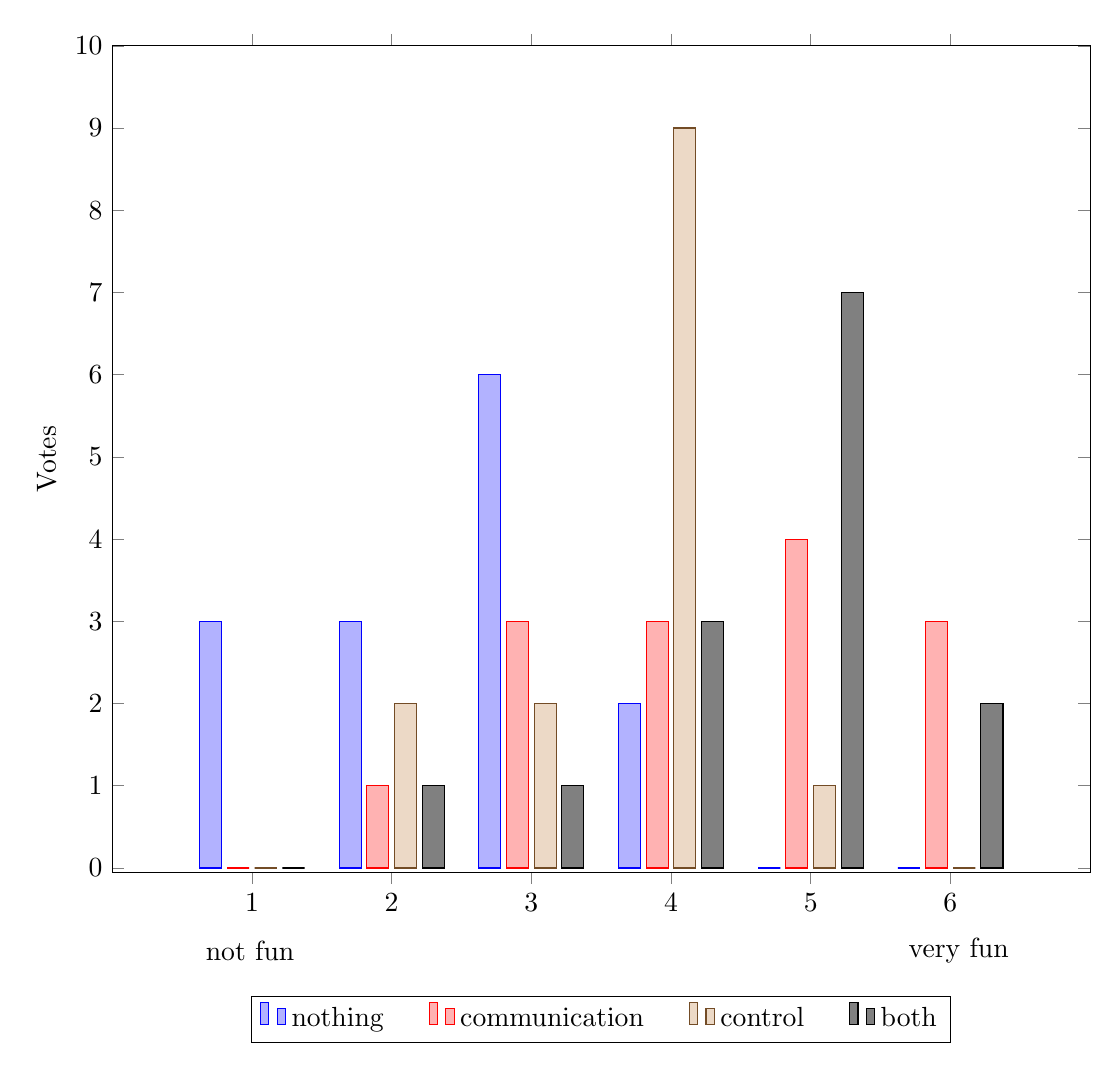
\begin{tikzpicture}
\begin{axis}[width=14cm,
	ylabel=Votes,
	ymin=-0.05,ymax=10,
	xmin=0,xmax=7,
	enlargelimits=false,
	xtick=data,
	legend style={at={(0.5, -0.15)},
		anchor=north, legend columns=-1,/tikz/every even column/.append style={column sep=0.5cm}},
	ybar,
	bar width=8pt,
]

% no control, no communication
\addplot
	coordinates {(1,3) (2,3) (3,6) (4,2) (5,0) (6,0)};

% no control, with communication
\addplot
	coordinates {(1,0) (2,1) (3,3) (4,3) (5,4) (6,3)};

% with control, no communication
\addplot
	coordinates {(1,0) (2,2) (3,2) (4,9) (5,1) (6,0)};

% with control, with communication
\addplot
	coordinates {(1,0) (2,1) (3,1) (4,3) (5,7) (6,2)};

\legend{nothing, communication, control, both};
\end{axis}
\node at (1.75,-1) {not fun};
\node at (10.75,-1) {very fun};
\end{tikzpicture}
\caption{Fun degree of the four scenarios}
\label{fig:results_fun}
\end{figure}

\def\scenarionames{{"None","Comm","Control","Comm+Cont"}}
\begin{figure}[htb]
	\centering
	\begin{tikzpicture}
		\begin{axis}[width=12cm,height=8cm,
			ylabel=Average,
			xmin=-1,xmax=4,
			ymin=0,ymax=6,
			enlargelimits=false,
			legend style={at={0.5, -0.15)},
				anchor=north, legend columns=-1,/tikz/every even column/.append style={column sep=0.5cm}},
			ybar,
			bar width=16pt,
			xtick=data,
			xticklabel={\pgfmathparse{\scenarionames[Mod(\tick,4)]}\pgfmathresult},
		]
			
			\addplot+[error bars/.cd,y dir=both,y explicit]
				coordinates {
					(0, 2.25) +- (0, 1.019)
					(1, 4.357) +- (0, 1.277)
					(2, 3.643) +- (0, 0.842)
					(3, 4.571) +- (0, 1.089)
				};

		\end{axis}

	\end{tikzpicture}
	\caption{Average vote with standard deviation}
	\label{fig:results_average}
\end{figure}

\subsection{RQ 1 Which type of bot is most fun to play with?}
``Which is most fun to play with, communicating bot, controllable bot, both communicating and
controllable bot, or none?'' Figure \ref{fig:results_fun} shows the questionnaire results from the
four questions, one for each scenario; the results are summorized in figure
\ref{fig:results_average} for an easier comparison.

To validate our hypothesis if the testers thought it was most fun to play (in this order) with a communicating and
controllable, communicating, controllable, and a bot with none of these features we conducted paired two-sample
T-tests, results found in table \ref{tbl:t-test-all}. These null hypotheses tests whether the
differences between the scenarios are enough to deduct
whether the order from figure \ref{fig:results_average} could be trusted.

\begin{table}[htbp]
\begin{center}
\begin{tabular}{|c|c|c|c|c|}
\hline
 & \textbf{None} & \textbf{Comm} & \textbf{Control} & \textbf{Comm+Cont} \\ \hline
\textbf{None} & N/A & 0.0013 & 0.0029 & 0.0015 \\ \hline
\textbf{Comm} & 0.0013 & N/A & 0.1461 & 0.6301 \\ \hline
\textbf{Control} & 0.0029 & 0.1461 & N/A & 0.0094 \\ \hline
\textbf{Comm+Cont} & 0.0015 & 0.6301 & 0.0094 & N/A \\ \hline
\end{tabular}
\end{center}
\vspace{-12pt}
\caption{Paired two-sample t-test}
\label{tbl:t-test-all}
\end{table}
From table \ref{tbl:t-test-all} we can see that there is not enough difference between neither
communication + control and only communication nor only communication and only control. What we can
deduct from this is the possible order of fun in table \ref{tbl:order_fun} where 1 is most fun and 4 is
least fun.

\begin{table}[htb]
	\centering
	\begin{tabular}{|l|l|l|l|}
		\hline
		\textbf{1} & Communication + Control & Communication & \\ \hline
		\textbf{2} & Communication + Control & Communication & Control \\ \hline
		\textbf{3} & Communication & Control & \\ \hline
		\textbf{4} & None & & \\ \hline

	\end{tabular}
	\caption{Possible fun order from the t-tests}
	\label{tbl:order_fun}
\end{table}

An interesting observation was that some testers preferred communication over both control and
communication. During the interviews we found a correlation between control and player skill—players
with higher skill tended to prefer control whereas lower skill players became overwhelmed by all
tasks, including the control of the bot.





\paragraph{Control \& communication}
During the interviews 8 of 14 testers felt it was most fun to play with the bot when both
communication and control was enabled. Two of the tester could not decide whether only communication or both
communication and control was more fun, but one mentioned that s/he would liked control and
communication more than only communication if s/he had been better at the game. Below you can find
the testers' reasons why control and communication was most fun to play.
\begin{itemize}
	\item I could build up my army, order him to attack and join his attack.
	\item Easier to plan because he told me his plans.
	\item I could order him to attack where I attacked using the follow command.
	\item You get a direct response from him after an order—you know that something will happen.
	\item Nice to be able to control him.
	\item It was fun that he explained his strategies.
\end{itemize}

\paragraph{Communication only}
6 of 14 testers (including the two testers already mentioned that could not decide on whether only
communication or both communication and control was most fun) thought it was most fun to play with
the bot when it only had communication on. Below you can find the testers' reasons why communication
was most fun to play.
\begin{itemize}
	\item I already had a lot on my mind, controlling him was a bit too much for me.	
	\item Easier for me to plan because he told me his plans.
	\item I am lazy therefore it was easier to let the bot do the hard work.
\end{itemize}

\paragraph{Control only}
2 of 14 testers thought it was most fun to play only with control. Although these might not be
credible as for one tester it was the only game s/he won in the test and s/he told us that it was
only because of that it was most fun, otherwise s/he guessed it would be more fun with
communication. The other tester only thought control was most fun as it was the first scenario s/he
tested, otherwise s/he thought control and communication was most fun because ``it was easier to play
when I (the tester) can send attacks at the same time his and it gets easier to see what the bot
does'' (paraphrased), i.e. same reasons as other players who thought control and communication was most fun.

\subsection{RQ 1.1 Which features are most liked?}
Below the most liked features are shown in two lists, one containing general features and the other
specific commands they liked. As mentioned these can serve as guidelines for future work what
features shall be prioritized.
\paragraph{General liked features}
Most noteworthy is the communication which more than half of the testers commented on, more
specifically ``Fun to know what the bot is doing'' and ``Easier to plan because he told me his
plans.''
\begin{itemize}
	\item Communication
	\begin{itemize}
		\item He said why attacked, expanded, and so forth—I could learn from his strategies.
		\item Fun to know what the bot is doing.
		\item Easier to plan because he told me his plans.
		\item Feels more like team play when he is communicating.
		\item Direct response after ordering a command, then you knew if the bot would follow the command or not.
		\item It had humor, e.g. Leeeeroooooooy Jenkins message when attacking.
		\item Almost like playing with a real player.
		\item Asked player for help when under attack.
	\end{itemize}
	\item Uses same strategies as humans, such as attacking when expanding.
	\item Very good macro, always has much more units than me.
	\item Own initiative to do things.
	\begin{itemize}
		\item Followed me when I wanted to attack, even though I did not order him—feeling that I play with someone.
		\item Very good at expanding, and often.
		\item I could plan after how it acted and collaborate.
	\end{itemize}
	\item Coordinated defense—came and defended me when I needed help.
	\item It did not run its own race, I felt involved in its decisions.
	\item Built tanks—I could back with my units and the tanks would clear the enemy units.
	\item Its attack cleared the path for me.
\end{itemize}

\paragraph{Liked commands}
\begin{itemize}
	\item Follow
	\begin{itemize}
		\item Doubles the amount of army size at one place.
		\item I did not have to attack by myself.
		\item Easier to coordinate where he should attack.
	\end{itemize}
	\item Attack
	\begin{itemize}
		\item I do not have to attack at the same place with my army.
		\item He could clear the path for me.
		\item Easy to reinforce as one could spam the attack button.
		\item He always had an army, if he attacked I could support him with my smaller army.
		\item He decided where to attack and I could follow and attack somewhere close.
	\end{itemize}
	\item Expand
	\begin{itemize}
		\item I like to control the timing between when I attack and he shall expand.
		\item I could order him to expand twice if the opportunity came, or just to expand when he did not notice he could expand.
	\end{itemize}
	\item Scout
	\begin{itemize}
		\item I do not have to scout and that is good as I am lazy.
	\end{itemize}
\end{itemize}

\subsection{RQ 1.2 Which features are most disliked?}
Instead of asking what features the testers disliked, we asked what they disliked about BATS (notice
the removal of feature). Below is a list of all things they disliked about BATS.
\paragraph{General disliked features}
Almost all testers mentioned they were annoyed by BATS halting its army in choke points making it
impossible for them to pass.
\begin{itemize}
	\item The army halted in choke points and made it impossible for me to come through.
	\item Got stuck when moving to a place, he ran back and forth until he finally ran more too long
		to the other side—note: regroup behavior.
	\item It did not follow me very well—note: when the squad it followed became very small (1-2
		units) the player did not notice it had units that the bot followed with 30+ units.
	\item Bot asks for help when few units attack and he can easily handle it.
	\item Felt like it changed how good it was during each scenarios.
	\item He attacked cowardly, slow attack with siege tanks instead of just marching in and killing
		everything which he could do in most situations.
	\item Sends too many messages at the same time, maybe queue up messages instead?—note: sometimes
		the bot will decide to retreat, but decides to attack directly after and then expand
		because it is attacking, thus 3 messages are printed directly after each other which can
		confuse the player..
	\item Never had units for drops.
	\item When it dropped it did not function very well.
	\item A better scout that scouted bases and not random locations.
\end{itemize}

\paragraph{Disliked commands}Two answered drop as it did not work properly, but most of the testers did not test all commands and thus could not answer if they disliked any command.

\subsection{RQ 1.3 Which features are missing?}
The testers were asked which features they missed during their scenarios, the first list presented
includes general features whereas the second list are specific commands they missed. These can serve
as guidelines for future developers what players want from a teammate bot.
\paragraph{General missed features}
\begin{itemize}
	\item More strategies, e.g. rush attacks, and would know about timings to make use of them.
	\item Use a variety of strategies depending on my build order.
	\item Give resources to the bot.
	\item Did not specify where he is under attack, would help me find the place.
	\item BATS could communicate what it thinks the player should do when s/he does not know what to do.
	\item More variety of units, more detection units.
	\item Scans in enemy bases.
	\item For the bot to play other races than Terran.
\end{itemize}

\paragraph{Missed commands, or improved existing commands}
\begin{itemize}
	\item A help button when the bot shall come and help me.
	\item Using way points for attacks to specify from where he should attack, either to not block my path or to create a more advanced attack.
	\item Drunken mode, random behavior.
	\item Command buttons grayed out when player could not use them.
	\item Retreat command.
	\item Abort command to abort the last command if the player misclicked.
	\item Hold position.
\end{itemize}

\subsection{Other questions and comments}
\paragraph{What surprised you in a positive way?}
A common misconception was that the testers would play against the bot and not with it. They thought
BATS was a good bot, that built up his army fast and that the tester did not need to babysit it.
They tended to like the funny messages, especially Leeeeeerrooooooy Jenkins. Common for many testers
were that the bot expanded just before they were going to send the expand command, which made them
think the bot was good at expanding and had a good timing on expands. A tester liked the underlying
reason behind each intention and not just the intention as s/he could learn from this. Another
tester was surprised by that it worked so well to play with a bot as they can be quite stupid.

\paragraph{What surprised you in a negative way?}
More than half of the testers thought BATS crowded the places he attacked and made it impossible to
bypass unless you had air units, 2 testers even changed their strategy to only air units because of
this. He did not clear the entire base as humans would do, but left the base when few buildings were
left. Twice the bot expanded to a location the player already expanded to, i.e. build a command
center beside their command center (or equal building). Sometimes the bot followed a small army
consisting of 1-2 units, this surprised the player as s/he thought it would either retreat or continue
attacking on its own.

\paragraph{If you won or lost, did you think it was because of you, BATS, or both?}
This question was not asked until the 6th tester, thus only 8 of 14 testers were asked this
question. Four of the tester thought they won because of both, where one of these thought it was
because of him/her in one of the four scenarios. Their reasons were that BATS was better at building
units, but they themselves had a better idea of strategy, where and how to attack. Two of the
testers thought it always because of them as they felt better than BATS, these two were amongst the
better players and also preferred control—a side note, there were two other players just as good as
them, one of them thought it was because of both and strangely the other thought it was because of
the bot. Another tester thought they won because of the bot as it had saved him/her at a very
crucial moment.

Only one loss occurred for the last 8 tester. The tester who lost felt that it was entirely
his/her fault as the bot had been attacked for 4 minutes and was defeated before the tester even
noticed it, although s/he mentioned that if the bot had said it was under attack it would never have
happened.

\paragraph{Commands used}
We noticed that many of the testers did not use all commands, no-one used the transition command as
all felt the bot handled that fairly well. Only a few (2–4) used the drop, expand, and scout
commands, with the same reason here as they felt the bot did a good job on this, except drop but
they did not feel as a drop was needed.

\paragraph{Other noteworthy comments}
One tester mentioned the bot felt like Brother in Arms where you can control other units. Another
tester mentioned that it was more fun to play with this bot than any other s/he had played with. A
third tester thought BATS could be used either when one wanted to play a regular co-op game but did
not have any friend to play with, or to fill an uneven team when playing with friends.

\subsection{Questions and comments about the experiment}
These are questions asked about the experiment itself and not directly associated with the bot.

\paragraph{Was the experiment fun or boring, and why?}
All testers thought it was fun to test the bot, both because StarCraft is a fun game and because it
was a new experience for many to play with a bot that you could control and communicate.

\paragraph{Was the experiment too long?}
The experiment was estimated to take 2 hours. Some testers thought it sounded quite long, but none
of the testers thought it was too long. Their reasons were that the scenarios were short (max 20
minutes) and they had fun testing the bot making time pass very quickly.

\paragraph{Other comments}
A tester commented how much difference there were between bots with and without communication, put
in the testers own words: ``I noticed how important the communication was and how bad something can
be when a feature is missing.''\footnote{Translated from Swedish ``Jag märkte hur viktig
kommunikationen var och hur dåligt någonting kan vara utan en feature.''}

% !TEX root = ../main.tex
\chapter{Related work}
% !TEX root = ../main.tex
% !TEX spellcheck = en_US
\chapter{Conclusions and future work}
First we go through our conclusions on the bot, what the players thought, liked and disliked about
the bot and scenarios. Then we go through some lessons we have learned during the project we thought
was worth mentioning, and last future work for researchers focusing on three different areas,
teammate bot behavior, communication and control.

\section{Bot conclusions}
We conclude that a teammate bot for RTS games that communicates its intentions and reasons is indeed
more fun to play with, although we did not find any statistical difference between Communication +
Control and only Communication both of these include communication.

What surprised us was that some players
preferred when the bot only communicated. This was later identified to depend on the player's skill
where more experienced players liked the ability to control the bot whereas beginners tended to get
overwhelmed by all the existing game action and thus did not want to focus on yet another task:
controlling the bot. This is an interesting question on how to balance the control so that
beginners aren't overwhelmed but at the same time meets the needs of a more skillful player. We talk
more about this in Future work \ref{sec:future_control}.\\


The most liked feature was the ability for the bot to communicate its intentions and reasons to the
player. The most reasons were ``it was fun to know what the bot is doing'' and ``easier to plan
because he told me his plans''. This aligns with what Norman states, humans want to know what the AI
is doing\cite{norman07}.

An important aspect BATS missed was point 5 from McGee's and Abraham's definition\cite{mcgee10} of a
real-time teammate bot, ``whenever possible, prioritizing the player experience''—for the full list
see section \ref{sec:teammate_bots}. When the player either ordered BATS to attack or follow
him/her, BATS almost always ended up blocking the path for the player close to the attack location,
not prioritizing the player experience as it should let the player through.
Disrespecting this ``rule'' probably made ``The army halted in choke points and made it impossible
for me to come through'' top the disliked features list.

\section{Project conclusions}
\paragraph{Magnusson's notes}
Being a perfectionist is not easy, this was one of the causes why we did not meet our first
deadline. I implemented features that were never used but what I thought were nice to have, such as
the Wait Goals, advanced drop mechanics, while we remove Wait goals and drops entirely and it would
not affect the test results.  In addition to this I changed existing systems much more than
needed—instead of using the existing squad manager with squads I create a new squad manager, this
was because the functionality differed quite much what we wanted to have in BATS, but maybe not
needed. We would have saved some weeks on this task alone.

In addition I tweaked and fixed small thing that ``it will only take two hours'', but I found many
of these small tweaks and some of them took more than two hours. After half the bot had been
implemented and the deadline was close, we decided to decrease the number of features and aim for
the next deadline, almost three months later. Now instead for fixing all small bugs and tweaks I
created a ticket in our project manager, then I forced myself to not work on them until all the
bot's main features were implemented. This worked much better and the bot was done, maybe not in no
time, but much faster.

In essence what I learned was that task prioritization is a must if one wants to finish a project,
and then only work on those assigned tasks, if new tasks were found one shall not do them directly
but either put them in the right priority or put them in a bag of things to do if there is time
left.

\section{Future work}
We will split the section in three parts, first discussing future work for the behavior of a
teammate bot, then improvements on the communication, and finally the control of a teammate bot.
While these are RTS game specific topics many of the Communication and Control topics can be
slightly changed to match another game genre.

\subsection{Teammate bot behavior}
BATS behaves in ways that we thought would be good, both through own experience, research, and
testing; but it still lacks a solid behavior to be used in a commercial game as its behavior does
not change depending on the play style of the human player. More research needs to be done on what
players want a teammate bot to do and how much initiative the bot shall have, if the bot has control
the degree of initiative can depend on how much the player want to control the bot, i.e. the more
control the player wants the less initiative the bot shall have, or does the players, independent of
skill and play style, always want the same initiative?

A possibility for teammate bots can be either a full-time or temporarily replacement for a human
player in online matches—temporarily when the player disconnects. But how shall the bot behave when
it is used as a replacement for the entire game? It needs to be balanced so it either matches the
human players' skills in its own team or by setting a predefined skill to either increase or
decrease the entire team's total skill.  When it acts as a temporarily replacement the players might
want it to continue using the same strategy as the player and not do any hasty actions that could
make the player loose, the bot could use some learning algorithm that always is on when the player
plays matches and then send out this information to the other clients if the player gets
disconnected, one of the clients could then take temporary control of the player continue play as
nothing happened.  For both scenarios it might be good to do player modeling for the teammate bot to
know how it shall play, further resources on player modeling for RTS games can be found
here\cite{bakkes09, jansen07, kabanza10, schadd07, synnaeve11}.

\subsection{Communication}
The messages from BATS are very simple and aimed to feel like less auto-generated messages. In case
of text messages the player might not want long ``human-like'' sentences, but instead short
sentences.

There is also the possibility to either synthesize the message or record own messages to see if the
player prefer messages that are read to him/her.  Reading messages out loud might be good but cannot
be processed as quickly by the player and it can be hard if the computer want to send messages very
often, meaning some research needs to be done on how often and what type of messages shall be sent
for the player not to be overwhelmed by messages—this type of research can also be done on text
messages.

\subsection{Control}
\label{sec:future_control}
We concluded that not all commands were used and players preferred control depending on their skill.
One could research which type of commands are preferred and how often they are issued. This could
then serve as another research where more control functionality is either displayed for a player
depending on his/her skill level, this could for example be used in campaigns where players get
introduced to new functionality in the teammate continuously during the campaign, just as s/he is
with new units.

Another experiment could be made how much level of detail the player wants over the commands. E.g.
shall attack make the bot attack at some place (as it does now), shall the player have the ability
to specify where it shall attack, shall the player have the ability to specify which path the attack
shall use, or where the attack shall wait before it reaches its destination for a simultaneous
attack?  This level of degree probably depends on the skill of the player, but as you might have
thought of now this can cause the player to simply play two players, but s/he only needs to control
one bot. This leads to yet another research for a new genre.

Research a new type of RTS genre where the player simply tell the bot what to do, i.e. the player
control the bot entirely but has setup some rules what it should build and how it behaves. This
would be more like a strategy/tactic game where the player neither need good macro or micro, but
good strategy and tactics.

As mentioned further research needs to be done when using the teammate bot as a replacement for
human players in online matches. In regard to control it might be difficult to select who shall
control the bot, or if everyone can control it?

%\appendix

%%  \include the `end matter'

%
% New style of Bibliography
% http://amath.colorado.edu/documentation/LaTeX/reference/faq/bibstyles.html
%
\bibliographystyle{plain}	% (uses file "IEEE.bst")
\bibliography{bibliography}	% expects file "thesis.bib"
%
%\input{glossary}
%\input{index}
%\input{guide_symbols}
%\input{guide_curriculum}

%%  finally, \include the list of previous bth-CS dissertations

%\cleardoublepage % if you are so inclined
%\include{bthcsdissertations} %PERSONALIZE that is: make sure you have the
%latest list.
%\include{guide_back1} % for a thesis with a back-flap summary
%\include{guide_back} %or take this one for a fairly plain back cover
 
\end{document}
